\ifx\type\undefined
  \documentclass[10pt, t]{beamer}
  \setbeamertemplate{footline}[page number]
\else
  \documentclass[10pt]{article}
  \usepackage[margin=1in]{geometry}
\fi

\usepackage{amsmath}
\usepackage{amssymb}
\usepackage{amsthm}
\usepackage{bbm}
\usepackage{cancel}
\usepackage{listings}
\usepackage{mathrsfs}
\usepackage{multirow}
\usepackage{soul}
\usepackage{stmaryrd}
\usepackage{tikz}
\usepackage{tikz-cd}
\usepackage{wrapfig}

\newtheorem*{algorithm}{Algorithm}
\newtheorem*{assumptions}{Assumptions}
\newtheorem*{conjecture}{Conjecture}
\newtheorem*{consequences}{Consequences}
\newtheorem*{exercise}{Exercise}
\newtheorem*{formalisation}{Formalisation}
\newtheorem*{proposition}{Proposition}
\newtheorem*{question}{Question}
\newtheorem*{remark}{Remark}

\ifx\type\undefined\else
  \newtheorem*{definition}{Definition}
  \newtheorem*{example}{Example}
  \newtheorem*{lemma}{Lemma}
  \newtheorem*{theorem}{Theorem}
\fi

\definecolor{keywordcolor}{rgb}{0.7, 0.1, 0.1}
\definecolor{tacticcolor}{rgb}{0.0, 0.1, 0.6}
\definecolor{commentcolor}{rgb}{0.4, 0.4, 0.4}
\definecolor{symbolcolor}{rgb}{0.0, 0.1, 0.6}
\definecolor{sortcolor}{rgb}{0.1, 0.5, 0.1}
\definecolor{attributecolor}{rgb}{0.7, 0.1, 0.1}
\def\lstlanguagefiles{lstlean.tex}
\lstset{language=lean}

\newcommand\A{\mathbb{A}}
\newcommand\C{\mathbb{C}}
\newcommand\F{\mathbb{F}}
\newcommand\G{\mathbb{G}}
\renewcommand\H{\mathbb{H}}
\newcommand\I{\mathbb{I}}
\newcommand\N{\mathbb{N}}
\renewcommand\P{\mathbb{P}}
\newcommand\Q{\mathbb{Q}}
\newcommand\R{\mathbb{R}}
\newcommand\Z{\mathbb{Z}}

\renewcommand\AA{\mathcal{A}}
\newcommand\BB{\mathcal{B}}
\newcommand\CC{\mathcal{C}}
\newcommand\DD{\mathcal{D}}
\newcommand\EE{\mathcal{E}}
\newcommand\FF{\mathcal{F}}
\newcommand\GG{\mathcal{G}}
\newcommand\HH{\mathcal{H}}
\newcommand\II{\mathcal{I}}
\newcommand\LL{\mathcal{L}}
\newcommand\MM{\mathcal{M}}
\newcommand\NN{\mathcal{N}}
\newcommand\OO{\mathcal{O}}
\newcommand\PP{\mathcal{P}}
\newcommand\RR{\mathcal{R}}
\renewcommand\SS{\mathcal{S}}
\newcommand\TT{\mathcal{T}}
\newcommand\XX{\mathcal{X}}

\renewcommand\aa{\mathfrak{a}}
\newcommand\cc{\mathfrak{c}}
\newcommand\dd{\mathfrak{d}}
\newcommand\ff{\mathfrak{f}}
\renewcommand\gg{\mathfrak{g}}
\newcommand\mm{\mathfrak{m}}
\newcommand\pp{\mathfrak{p}}
\newcommand\qq{\mathfrak{q}}
\renewcommand\ss{\mathfrak{s}}

\newcommand\LLL{\mathscr{L}}

\newcommand\ab{\mathrm{ab}}
\newcommand\Ab{\mathbf{Ab}}
\newcommand\Alg{\mathbf{Alg}}
\newcommand\Aff{\mathbf{Aff}}
\newcommand\Aut{\operatorname{Aut}}
\newcommand\Az{\mathrm{Az}}
\newcommand\Br{\operatorname{Br}}
\newcommand\BSD{\operatorname{BSD}}
\newcommand\ch{\operatorname{char}}
\newcommand\Cl{\operatorname{Cl}}
\newcommand\coker{\operatorname{coker}}
\newcommand\cris{\mathrm{cris}}
\renewcommand\d{\mathrm{d}}
\newcommand\Div{\operatorname{Div}}
\newcommand\dR{\mathrm{dR}}
\newcommand\EN{\operatorname{EN}}
\newcommand\End{\operatorname{End}}
\newcommand\ES{\operatorname{ES}}
\newcommand\et{\mathrm{\acute{e}t}}
\newcommand\Et{\mathbf{\acute{E}t}}
\newcommand\Ext{\operatorname{Ext}}
\newcommand\Fr{\operatorname{Fr}}
\newcommand\Frac{\operatorname{Frac}}
\newcommand\Gal{\operatorname{Gal}}
\newcommand\GL{\operatorname{GL}}
\newcommand\Gr{\mathrm{Gr}}
\newcommand\Hom{\operatorname{Hom}}
\newcommand\HT{\mathrm{HT}}
\newcommand\id{\operatorname{id}}
\newcommand\im{\operatorname{im}}
\newcommand\Ind{\operatorname{Ind}}
\renewcommand\inf{\operatorname{inf}}
\newcommand\inv{\operatorname{inv}}
\newcommand\Irr{\operatorname{Irr}}
\newcommand\Jac{\operatorname{Jac}}
\newcommand\lcm{\operatorname{lcm}}
\newcommand\Mat{\operatorname{Mat}}
\newcommand\Mod{\mathbf{Mod}}
\newcommand\Nm{\operatorname{Nm}}
\newcommand\nr{\mathrm{nr}}
\newcommand\NS{\operatorname{NS}}
\newcommand\Ob{\operatorname{Ob}}
\newcommand\ord{\operatorname{ord}}
\newcommand\op{\mathrm{op}}
\newcommand\PGL{\operatorname{PGL}}
\newcommand\Pic{\operatorname{Pic}}
\newcommand\Prob{\operatorname{Prob}}
\newcommand\Proj{\operatorname{Proj}}
\newcommand\PSh{\mathbf{PSh}}
\newcommand\Reg{\operatorname{Reg}}
\newcommand\res{\operatorname{res}}
\newcommand\rk{\operatorname{rk}}
\newcommand\Sch{\mathbf{Sch}}
\newcommand\Sel{\operatorname{Sel}}
\newcommand\Set{\mathbf{Set}}
\newcommand\sgn{\operatorname{sgn}}
\newcommand\Sh{\mathbf{Sh}}
\newcommand\SL{\operatorname{SL}}
\newcommand\Spec{\operatorname{Spec}}
\newcommand\supp{\operatorname{supp}}
\newcommand\Tam{\operatorname{Tam}}
\newcommand\Top{\mathbf{Top}}
\newcommand\tor{\operatorname{tor}}
\newcommand\tr{\operatorname{tr}}
\newcommand\tra{\operatorname{tra}}
\newcommand\WC{\operatorname{WC}}

\DeclareFontFamily{U}{wncyr}{}
\DeclareFontShape{U}{wncyr}{m}{n}{<->wncyr10}{}
\DeclareSymbolFont{cyr}{U}{wncyr}{m}{n}
\DeclareMathSymbol{\Sha}{\mathord}{cyr}{"58}

\newcommand{\function}[5][]{
  \if &#1&
    \begin{array}{rcl}
      #2 & \longrightarrow & #3 \\
      #4 & \longmapsto     & #5
    \end{array}
  \else
    \begin{array}{rcrcl}
      #1 & : & #2 & \longrightarrow & #3 \\
         &   & #4 & \longmapsto     & #5
    \end{array}
  \fi
}

\newcommand{\functions}[7][]{
  \if &#1&
    \begin{array}{rcl}
      #2 & \longrightarrow & #3 \\
      #4 & \longmapsto     & #5 \\
      #6 & \longmapsto     & #7 \\
    \end{array}
  \else
    \begin{array}{rcrcl}
      #1 & : & #2 & \longrightarrow & #3 \\
         &   & #4 & \longmapsto     & #5 \\
         &   & #6 & \longmapsto     & #7
    \end{array}
  \fi
}
\title{Teaching a computer algebraic number theory}
\subtitle{Algebra, Number Theory, Logic, and Representation Theory Seminar}
\author{David Kurniadi Angdinata}
\institute{London School of Geometry and Number Theory}
\date{Tuesday, 25 March 2025}

\begin{document}

\frame\maketitle

\begin{frame}{Who am I?}

I am an aspiring algebraic number theorist in the final year of my PhD.

\bigskip My thesis will be on twisted L-functions of elliptic curves over global fields, which arise in equivariant Birch and Swinnerton-Dyer conjectures.

\bigskip In my first year, I was introduced to an interactive theorem prover called Lean, and tried to formalise the Mordell--Weil theorem as a mini-project.

\bigskip Over the past three years, I saw the potential: prominent mathematicians involved in collaborative projects, massive investments from multinational corporations and philanthropists, headlines of popular science journals.

\bigskip Today, I will share my thoughts so far:
\begin{itemize}
\item why do interactive theorem proving?
\item why do interactive theorem proving in Lean?
\item why do algebraic number theory in Lean?
\end{itemize}

\end{frame}

\begin{frame}{Interactive theorem proving}

Wikipedia says that an \textbf{interactive theorem prover} is a software tool to assist with the development of formal proofs by human–machine collaboration, which involves some sort of interactive proof editor, or other interface, with which a human can guide the search for proofs, the details of which are stored in, and some steps provided by, a computer.

\bigskip I think that \textbf{interactive theorem proving} is the experience of writing mathematics in a rigorous language understood by a computer.

\bigskip This includes axioms, definitions, theorems, proofs, and even techniques.

\bigskip Behind the scenes, the compiler does some magic in the \emph{kernel} to assess the validity of the mathematics, akin to the role of journal reviewers.

\bigskip In this sense, formalisations in interactive theorem provers are \emph{verified}, in contrast to computer algebra systems like Magma and SageMath.

\end{frame}

\begin{frame}[fragile]{Basic example}

Here is a theorem in Lean that $ \im(f) \le \ker(f) $ whenever $ g \circ f = 1 $.

\begin{lstlisting}[basicstyle=\scriptsize, frame=single]
variable {A B C : Type} [Group A] [Group B] [Group C]

def ker (f : A →* B) : Subgroup A where
  carrier  := {a : A | f a = 1}
  one_mem' := by simp
  inv_mem' := by simp
  mul_mem' := by aesop

def im (f : A →* B) : Subgroup B where
  carrier  := {b : B | ∃ a : A, b = f a}
  one_mem' := ⟨1, by simp⟩
  inv_mem' := fun ⟨a, _⟩ ↦ ⟨a⁻¹, by aesop⟩
  mul_mem' := fun ⟨a, _⟩ ⟨b, _⟩ ↦ ⟨a * b, by aesop⟩

theorem im_le_ker {f : A →* B} {g : B →* C} (h : ∀ a : A, g (f a) = 1) :
    im f ≤ ker g := by    -- Goal is ∀ b : B, (∃ a : A, b = f a) → (g b = 1)
  intro b hb                 -- Goal is g b = 1
                                 -- New hypotheses (b : B) (hb : ∃ a : A, (b = f a))
  rcases hb with ⟨a, ha⟩ -- Goal is g b = 1
                                 -- New hypotheses (b : B) (a : A) (ha : b = f a)
  rewrite [ha]               -- Goal is g (f a) = 1
  exact h a                   -- No goals!
\end{lstlisting}

\end{frame}

\begin{frame}{Notable examples}

Historically, they were used to check proofs that drew scepticism.
\begin{itemize}
\item The proof of the four colour theorem by Appel and Haken (1976) involved analysing 1834 reducible configurations of maps manually. Gonthier et al (2005) formalised it in Coq.
\item The proof of the odd order theorem by Feit and Thompson in 1960 involved complicated arguments in group theory spanning 255 pages. Gonthier et al (2012) formalised it in Coq.
\item The proof of the Kepler conjecture by Hales (1998) involved solving 100000 linear programming problems. Hales started the \textbf{Flyspeck project} (2003) to formalise it in Coq, and completed it in \emph{11 years}.
\item The field of condensed mathematics was developed by Clausen and Scholze (2019). Scholze started the \textbf{liquid tensor experiment} (2020) to formalise a technical lemma on liquid vector spaces in Lean, and Commelin et al completed it in \emph{20 months}.
\item The polynomial Freiman--Ruzsa conjecture was proven by Gowers, Green, Manners, and Tao (Nov 2023). Tao started a formalisation project in Lean 4 days later, and completed it in \emph{3 weeks}.
\end{itemize}

\end{frame}

\begin{frame}{Current motivations}

Nowadays, they have evolved to serve many other purposes.
\begin{itemize}
\item They allow for large-scale collaborations, akin to Gowers's Polymath Project, but organisation is done via a version control system, and the human moderator is replaced with the language compiler. Example: Tao's \textbf{equational relations} project.
\item They train artificial intelligence by verifying arguments generated by neural networks when presented with mathematical problems. Example: Google Deepmind's \textbf{AlphaProof} model.
\item They build self-consistent databases of mathematics for search engines, akin to de Jong's Stacks Project in algebraic geometry. Example: Peking University BICMR's \textbf{LeanSearch} engine.
\item They present surprising artifacts, such as unnecessary assumptions, simplification of arguments, or even issues in existing literature. Example: Chambert-Loir and de Frutos-Fern\'andez discovered an incorrect lemma in a fundamental paper on divided power structures (Dec 2024), which temporarily \emph{broke crystalline cohomology}!
\item They are \emph{fun}! Example: I am addicted.
\end{itemize}

\end{frame}

\begin{frame}{Lean theorem prover}

\begin{wrapfigure}[3]{r}{0.2\textwidth}
\includegraphics[width=0.2\textwidth]{img/lean.png}
\end{wrapfigure}

Lean is one of the many interactive theorem provers commonly used for formalising pure mathematics: Isabelle, HOL Light, Coq, Metamath, Mizar, etc.

\bigskip The first version of Lean was launched in 2013 by Leonardo de Moura at \emph{Microsoft Research} and later at \emph{Amazon Web Services}, with current development supported by the \emph{Lean Focused Research Organisation}.

\bigskip The current version of Lean uses a \emph{dependent type theory} called \emph{calculus of constructions with inductive types}, unlike Isabelle and HOL Light.

\bigskip Furthermore, it is also a \emph{functional programming language}, written in C++ and \emph{Lean}, with support for \emph{multithreading} and \emph{metaprogramming}.

\bigskip Finally, it supports \emph{Unicode symbols}, and can be run in \emph{common editors} like Visual Studio Code, Emacs, and Neovim.

\end{frame}

\begin{frame}{Lean's mathematical community}

I think the main appeal of Lean is its mathematical community, which arose from \emph{purely sociological} factors: cleanliness of language syntax, good communication with developers, amazing support from community, launch of collaborative projects, interest from Fields Medallists, etc.

\bigskip As a result, the community embarked on many collaborative projects:
\begin{itemize}
\item perfectoid spaces by Buzzard, Commelin, and Massot (2018 -- 2020)
\item sphere eversion by Massot, Nash, and van Doorn (2020 -- 2023)
\item Fermat's last theorem for regular primes by Best, Birkbeck, Brasca, Rodriguez, van de Velde, and Yang (2023 -- 2024)
\item local class field theory by de Frutos-Fern\'andez and Nuccio (Sep 2022 --)
\item prime number theorem and... led by Kontorovich (Jan 2024 --)
\item analytic number theory exponent database led by Tao (Aug 2024 --)
\item infinity cosmos led by Riehl (Sep 2024 --)
\item Fermat's last theorem led by Buzzard (Oct 2024 --)
\end{itemize}

\end{frame}

\begin{frame}{Lean's mathematical library}

Large formalisation projects are enabled by Lean's mathematical library \texttt{mathlib}, which is completely \emph{monolithic} and emphasises \emph{generality}.

\bigskip Currently, \texttt{mathlib} is a graduate student in algebra, and knows:
\begin{itemize}
\item linear algebra: matrices, projective modules, Clifford algebras, Hopf algebras, Lie algebras, ordinary representation theory
\item field theory: finite fields, function fields, finite Galois theory, absolute Galois groups, central division algebras, Ax--Grothendieck theorem
\item group theory: symmetric groups, structure theorems, Sylow theorems, nilpotent groups, primitive groups, finitely generated groups, free groups, Coxeter groups, abelian group cohomology
\item ring theory: domains, localisation, primary decomposition, integral closure, chain conditions, graded modules, Henselian rings, modules of differentials, basic dimension theory, basic homological algebra
\item algebraic geometry: schemes, morphism properties, valuative criteria, coherent sheaves, sheaf cohomology, Grothendieck topologies
\end{itemize}

\end{frame}

\begin{frame}{Algebraic number theory in Lean}

In particular, \texttt{mathlib} also knows some non-trivial results in number theory, which is fundamentally \emph{applied} pure mathematics, including:
\begin{itemize}
\item elementary theory: Lagrange's theorem on sums of four squares, Legendre's theorem on rational approximation, Gauss's law of quadratic reciprocity, Bertrand's postulate
\item analytic theory: Dirichlet's theorem on primes in arithmetic progressions, Liouville's theorem on transcendental numbers, boundedness of Eisenstein series, functional equation of Hurwitz $ \zeta $-functions, Gallagher's ergodic theorem, the Selberg sieve
\item local theory: Hensel's lemma for $ \Q_p $, ramification--inertia formula, basic properties of ad\`ele rings, basic properties of Witt vectors
\item global theory: Ostrowski's theorem for $ \Q $, product formula, finiteness of class numbers, Dirichlet's unit theorem, Galois group of cyclotomic extensions, Kummer--Dedekind theorem
\item Diophantine functions and Matiyasevic's theorem
\item Fermat's last theorem for exponent $ 3 $ and $ 4 $ and for polynomials
\end{itemize}
It will be learning about class field theory in July!

\end{frame}

\begin{frame}{Elliptic curves in Lean}

Since 2021, I have been formalising an \emph{algebraic} theory of elliptic curves.

\bigskip However, \texttt{mathlib} does not know what a curve is! This is actually fine, because the Riemann--Roch theorem gives an equivalence of categories
$$ \{\text{elliptic curves over} \ F\} \cong \left\{\begin{array}{c} \text{tuples} \ (a_1, a_2, a_3, a_4, a_6) \in F^5 \\ \text{such that} \ \Delta(a_i) \ne 0 \end{array}\right\}, $$
for any field $ F $. Currently \texttt{mathlib} thinks that
\begin{itemize}
\item an elliptic curve $ E $ over a ring $ R $ is the data of a tuple $ (a_1, a_2, a_3, a_4, a_6) \in R^5 $ and a proof that $ \Delta(a_i) \in R^\times $, and
\item a point on $ E $ is either $ \OO $ or a tuple $ (x, y) \in R^2 $ such that
$$ y^2 + a_1xy + a_3y = x^3 + a_2x^2 + a_4x + a_6. $$
\end{itemize}
The algebra can be developed independently of the geometry!

\bigskip How far can we develop the arithmetic purely algebraically?

\end{frame}

\begin{frame}{The group law in Lean}

By construction, this means that the geometric addition law is given by explicit rational functions, and associativity is known to be \emph{very difficult}. Generically, an equality of the $ X $-coordinates of $ (P + Q) + R $ and $ P + (Q + R) $ is an equality of multivariate polynomials with 26,082 terms!

\bigskip Classically, Riemann--Roch gives an explicit bijection from $ E(F) $ to the degree-zero divisor class group $ \Pic_F^0(E) $ that preserves the addition law. While \texttt{mathlib} does not know about divisors, it does know that integral domains $ D $ have ideal class groups $ \Cl(D) $, which translates to a map
$$ \functions{E(F)}{\Cl(F[E])}{\OO}{[(1)]}{(x, y)}{[(X - x, Y - y)]}. $$
In 2022, Junyan Xu discovered an elementary but novel proof that this map is injective, \emph{due to limitations in \texttt{mathlib}}. I formalised his argument in Lean and we wrote a paper that was published in ITP 2023.

\end{frame}

\begin{frame}{The $ n $-torsion subgroup in Lean}

The fundamental theorem in the \emph{arithmetic} of elliptic curves is the fact that $ E_{\overline{F}}[n] $ is a rank two module over $ (\Z / n)[G_F] $ whenever $ \ch(F) \nmid n $.

\bigskip Thus the $ \ell $-adic Tate module $ T_\ell E_{\overline{F}} := \varprojlim_n E_{\overline{F}}[\ell^n] $ is a two-dimensional $ \ell $-adic Galois representation, which is crucial in Tate's isogeny theorem, Serre's open image theorem, Wiles's modularity lifting theorem, etc.

\bigskip The Arithmetic of Elliptic Curves by Silverman attempts to prove this in Exercise 3.7 in seven parts, providing explicit inductive definitions of certain division polynomials $ \psi_n, \phi_n, \omega_n \in F[X, Y] $ in terms of $ a_i \in F $.

\bigskip Exercise 3.7(d) claims that for any point $ (x, y) \in E(F) $,
$$ [n]((x, y)) = \left(\dfrac{\phi_n(x, y)}{\psi_n(x, y)^2}, \dfrac{\omega_n(x, y)}{\psi_n(x, y)^3}\right). $$
The key idea is that $ \psi_n(x, y) = 0 $ occurs precisely when $ [n]((x, y)) = \OO $.

\end{frame}

\begin{frame}{The multiplication-by-$ n $ formula in Lean}

\begin{conjecture}
No one has done Exercise 3.7 purely algebraically.
\end{conjecture}

\begin{proof}
\renewcommand\qedsymbol{}
\begin{itemize}
\item Exercise 3.7(c) that $ (\phi_n, \psi_n^2) = 1 $ needs Exercise 3.7(d).
\item Definition of $ \omega_n $ is \emph{incorrect}! It should instead be
$$ \omega_n := \tfrac{1}{2}\left(\psi_{2n} / \psi_n - a_1\phi_n\psi_n - a_3\psi_n^3\right). $$
\item Integrality of $ \omega_n $ needs Exercise 3.7(g) that $ \psi_n $ is an elliptic sequence
$$ \psi_{n + m}\psi_{n - m}\psi_r^2 = \psi_{n + r}\psi_{n - r}\psi_m^2 - \psi_{m + r}\psi_{m - r}\psi_n^2. $$
\item Exercise 3.7(g) needs the stronger result that $ \psi_n $ is an elliptic net
$$ \psi_{n + m}\psi_{n - m}\psi_{r + s}\psi_{r - s} = \psi_{n + r}\psi_{n - r}\psi_{m + s}\psi_{m - s} - \psi_{m + r}\psi_{m - r}\psi_{n + s}\psi_{n - s}. $$
\item Exercise 3.7(d) needs four special cases of this stronger result. $ \square $
\end{itemize}
\vspace{-0.5cm}
\end{proof}

\end{frame}

\begin{frame}{The $ \ell $-adic Tate module in Lean}

Peiran Wu (
\begin{tikzpicture} \draw [fill=blue] (0, 0) rectangle (0.25, 0.25); \end{tikzpicture}), Junyan Xu (
\begin{tikzpicture} \draw [fill=magenta] (0, 0) rectangle (0.25, 0.25); \end{tikzpicture}), and I (
\begin{tikzpicture} \draw [fill=red] (0, 0) rectangle (0.25, 0.25); \end{tikzpicture}) formalised $ T_\ell E_{\overline{F}} \cong \Z_\ell^2 $ in Lean.

\begin{center}
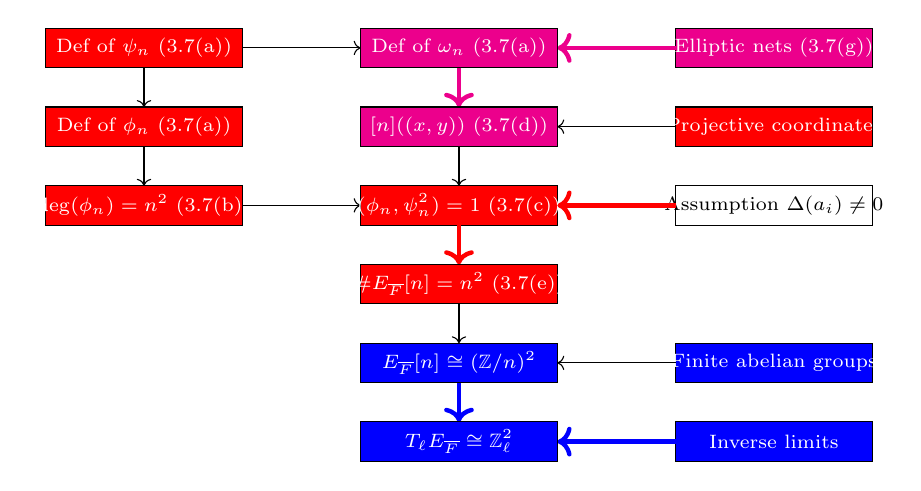
\begin{tikzpicture}
\draw [fill=red] (0, 0) rectangle node[color=white]{\scriptsize Def of $ \psi_n $ (3.7(a))} (2.5, -0.5);
\draw [->] (1.25, -0.5) to (1.25, -1);
\draw [fill=red] (0, -1) rectangle node[color=white]{\scriptsize Def of $ \phi_n $ (3.7(a))} (2.5, -1.5);
\draw [->] (1.25, -1.5) to (1.25, -2);
\draw [fill=red] (0, -2) rectangle node[color=white]{\scriptsize $ \deg(\phi_n) = n^2 $ (3.7(b))} (2.5, -2.5);
\draw [fill=red] (8, -1) rectangle node[color=white]{\scriptsize Projective coordinates} (10.5, -1.5);
\draw [->] (2.5, -0.25) to (4, -0.25);
\draw [fill=magenta] (8, 0) rectangle node[color=white]{\scriptsize Elliptic nets (3.7(g))} (10.5, -0.5);
\draw [->, color=magenta, ultra thick] (8, -0.25) to (6.5, -0.25);
\draw [fill=magenta] (4, 0) rectangle node[color=white]{\scriptsize Def of $ \omega_n $ (3.7(a))} (6.5, -0.5);
\draw [->, color=magenta, ultra thick] (5.25, -0.5) to (5.25, -1);
\draw [->] (8, -1.25) to (6.5, -1.25);
\draw [fill=magenta] (4, -1) rectangle node[color=white]{\scriptsize $ [n]((x, y)) $ (3.7(d))} (6.5, -1.5);
\draw [->] (5.25, -1.5) to (5.25, -2);
\draw [->] (2.5, -2.25) to (4, -2.25);
\draw [fill=red] (4, -2) rectangle node[color=white]{\scriptsize $ (\phi_n, \psi_n^2) = 1 $ (3.7(c))} (6.5, -2.5);
\draw [->, color=red, ultra thick] (5.25, -2.5) to (5.25, -3);
\draw [fill=red] (4, -3) rectangle node[color=white]{\scriptsize $ \#E_{\overline{F}}[n] = n^2 $ (3.7(e))} (6.5, -3.5);
\draw [->] (5.25, -3.5) to (5.25, -4);
\draw [fill=blue] (8, -4) rectangle node[color=white]{\scriptsize Finite abelian groups} (10.5, -4.5);
\draw [->] (8, -4.25) to (6.5, -4.25);
\draw [fill=blue] (4, -4) rectangle node[color=white]{\scriptsize $ E_{\overline{F}}[n] \cong (\Z / n)^2 $} (6.5, -4.5);
\draw [->, color=blue, ultra thick] (5.25, -4.5) to (5.25, -5);
\draw [fill=blue] (8, -5) rectangle node[color=white]{\scriptsize Inverse limits} (10.5, -5.5);
\draw [->, color=blue, ultra thick] (8, -5.25) to (6.5, -5.25);
\draw [fill=blue] (4, -5) rectangle node[color=white]{\scriptsize $ T_\ell E_{\overline{F}} \cong \Z_\ell^2 $} (6.5, -5.5);
\draw (8, -2) rectangle node{\scriptsize Assumption $ \Delta(a_i) \ne 0 $} (10.5, -2.5);
\draw [->, color=red, ultra thick] (8, -2.25) to (6.5, -2.25);
\end{tikzpicture}
\end{center}

Note that the assumption $ \Delta(a_i) \ne 0 $ is unnecessary until Exercise 3.7(c).

\end{frame}

\begin{frame}[c]{Future projects}

Can we formalise the \emph{full statement} of the Birch and Swinnerton-Dyer conjecture for an elliptic curve $ E $ over a number field $ K $ in Lean?

\begin{center}
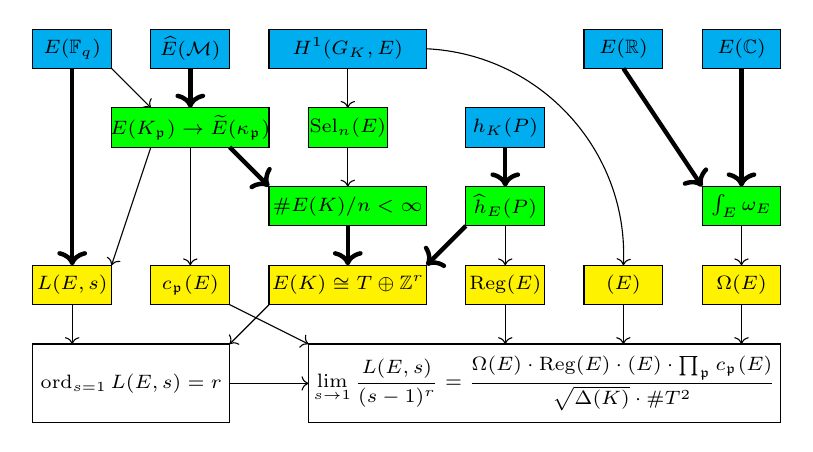
\begin{tikzpicture}
\draw [fill=cyan] (0, 0) rectangle node{\scriptsize $ E(\F_q) $} (1, -0.5);
\draw [->] (1, -0.5) to (1.5, -1);
\draw [fill=cyan] (1.5, 0) rectangle node{\scriptsize $ \widehat{E}(\MM) $} (2.5, -0.5);
\draw [->, ultra thick] (2, -0.5) to (2, -1);
\draw [fill=green] (1, -1) rectangle node{\scriptsize $ E(K_\pp) \to \widetilde{E}(\kappa_\pp) $} (3, -1.5);
\draw [->, ultra thick] (0.5, -0.5) to (0.5, -3);
\draw [->] (1.5, -1.5) to (1, -3);
\draw [fill=yellow] (0, -3) rectangle node{\scriptsize $ L(E, s) $} (1, -3.5);
\draw [->, ultra thick] (2.5, -1.5) to (3, -2);
\draw [fill=cyan] (3, 0) rectangle node{\scriptsize $ H^1(G_K, E) $} (5, -0.5);
\draw [->] (4, -0.5) to (4, -1);
\draw [fill=green] (3.5, -1) rectangle node{\scriptsize $ \Sel_n(E) $} (4.5, -1.5);
\draw [->] (4, -1.5) to (4, -2);
\draw [fill=green] (3, -2) rectangle node{\scriptsize $ \#E(K) / n < \infty $} (5, -2.5);
\draw [fill=cyan] (5.5, -1) rectangle node{\scriptsize $ h_K(P) $} (6.5, -1.5);
\draw [->, ultra thick] (6, -1.5) to (6, -2);
\draw [fill=green] (5.5, -2) rectangle node{\scriptsize $ \widehat{h}_E(P) $} (6.5, -2.5);
\draw [->, ultra thick] (4, -2.5) to (4, -3);
\draw [->, ultra thick] (5.5, -2.5) to (5, -3);
\draw [fill=yellow] (3, -3) rectangle node{\scriptsize $ E(K) \cong T \oplus \Z^r $} (5, -3.5);
\draw [->] (0.5, -3.5) to (0.5, -4);
\draw [->] (3, -3.5) to (2.5, -4);
\draw (0, -4) rectangle node{\scriptsize $ \ord_{s = 1} L(E, s) = r $} (2.5, -5);
\draw [->] (2, -1.5) to (2, -3);
\draw [fill=yellow] (1.5, -3) rectangle node{\scriptsize $ c_\pp(E) $} (2.5, -3.5);
\draw [->] (6, -2.5) to (6, -3);
\draw [fill=yellow] (5.5, -3) rectangle node{\scriptsize $ \Reg(E) $} (6.5, -3.5);
\draw [->] (5, -0.25) to [bend left=45] (7.5, -3);
\draw [fill=yellow] (7, -3) rectangle node{\scriptsize $ \Sha(E) $} (8, -3.5);
\draw [->] (2.5, -4.5) to (3.5, -4.5);
\draw [->] (2.5, -3.5) to (3.5, -4);
\draw [->] (6, -3.5) to (6, -4);
\draw [->] (7.5, -3.5) to (7.5, -4);
\draw (3.5, -4) rectangle node{\scriptsize $ \displaystyle\lim_{s \to 1} \dfrac{L(E, s)}{(s - 1)^r} = \dfrac{\Omega(E) \cdot \Reg(E) \cdot \Sha(E) \cdot \prod_\pp c_\pp(E)}{\sqrt{\Delta(K)} \cdot \#T^2} $} (9.5, -5);
\draw [fill=cyan] (7, 0) rectangle node{\scriptsize $ E(\R) $} (8, -0.5);
\draw [->, ultra thick] (7.5, -0.5) to (8.5, -2);
\draw [fill=cyan] (8.5, 0) rectangle node{\scriptsize $ E(\C) $} (9.5, -0.5);
\draw [->, ultra thick] (9, -0.5) to (9, -2);
\draw [fill=green] (8.5, -2) rectangle node{\scriptsize $ \int_E \omega_E $} (9.5, -2.5);
\draw [->] (9, -2.5) to (9, -3);
\draw [fill=yellow] (8.5, -3) rectangle node{\scriptsize $ \Omega(E) $} (9.5, -3.5);
\draw [->] (9, -3.5) to (9, -4);
\end{tikzpicture}
\end{center}

Come join the Lean community to enter a new era of mathematics!

\end{frame}

\end{document}